\documentclass[aspectratio=169,notheorems]{corvinusmetropolis}

\usepackage[hungarian]{babel}
\addbibresource{bibliography.bib}
\setbeamertemplate{frametitle continuation}{}

\renewcommand{\myinstlogo}{./corvinus-logos/color_simple_HUN.pdf}

\title{MNB csapatépítő szakmai előadás}
\subtitle{Biodiverzitás és Nature kockázat az európai piacon}
\author{Molnár Marcell\\Konzulens: Dr. Dömötör Barbara}
\email{marcell.molnar@stud.uni-corvinus.hu}

\institute[Corvinus University]
  {
  Pénzügy és számvitel alapszak\\
  Pénzügy specializáció\\
  Email: \putemail\\
  }
\date{2026. október 8.}
\titlegraphic{\hfill{\includegraphics[width=.2\textwidth]{\myinstlogo}}}
\keywords{biodiversity_finance, nature_finance, sustainable_finance}

\begin{document}
\simpleopen{}

\begin{frame}
  \frametitle{Irodalomi háttér}
  Az elmúlt években a Fenntartható Pénzügyek kutatói fokozott figyelmet fordított az új publikációkban a Biodiversity Finance ágnak\\ 
  Friss, releváns kutatások:
  \begin{itemize}
    \item \alert{biodiverzitási prémium} jelenléte és mértéke \parencite{coqueret_biodiversity_2024, naffa_biodiversity_2024}
    \item \alert{ENCORE adatbázis} biodiverzitás témakörben \parencite{clement_mapping_2025}
    \item \alert{private capital befektetések} \parencite{flammer_biodiversity_2025}\\
  \end{itemize}
  A hozzájárulásunk a szakirodalomhoz a biodiversity/nature hatások empirikus vizsgálata az európai részvénypiacon
\end{frame}

\begin{frame}
  \frametitle{Módszertan I.}
  A módszertanunk a Markowitz portfóliómodellre épül

  Egy olyan befektetőt feltételezünk (shortolás megengedett), akinek a hasznossági függvényébe a vagyon maximalizálása mellett, \alert{pozitívan gondolkodik a magasabb biodiversity/nature értékekről}.\\
  \pause
  \textcite{pedersen_responsible_2021} alapján a \alert{hasznossági fv-e lineáris és a következő alakú}:
  \metroset{block=fill}
  \begin{block}{Kiegészített hasznossági függvény}
  \begin{equation}
    U = E[\widehat{W}|s] - \frac{\hat{\gamma}}{2}Var(\widehat{W}|s) + Wf(\bar{s}),
  \end{equation}
  ahol a vagyonfüggvény $\widehat{W}=W\cdot(1+r^f+x'r)$, $\hat{\gamma}$ az abszolút kockázatelutasító paraméter, $s$ és $\bar{s}$ pedig a biodiversity/nature score és számtani átlaga*.
  \end{block}
  \textit{* $s$ az adott proxy értéket és $\bar{s}$ az átlagát jelöli!}
\end{frame}

\begin{frame}
  \frametitle{Módszertan II.}
  Egy sztenderd mean-variance hasznosságfüggvényű befektető a befektetési univerzumban megkeresi az \alert{érintési portfóliót}, majd ezt keveri a \alert{kockázatmentes eszközzel} az egyéni kockázatkerülésének függvényében.\\
  \pause
  \medskip
  Az érintési portfólió az a portfólió, ami a legmagasabb Sharpe-rátával rendelkezik. Ebből kiindulva \alert{ezt a koncepciót \textcite{pedersen_responsible_2021} általánosította} azzal, hogy \alert{minden egyes sztenderizált proxy mellett} (jelen esteben biodiversity score), \alert{meghatározható legyen a maximálisan elérhető Sharpe-ráta}.\\
  \pause
  \bigskip
  A probléma idáig nem függ az egyéni hasznosságtól, azaz a befektetési univerzumra egyértelműen meghatározható az ún. \imp{BIODIV-SR határ}!
\end{frame}

\begin{frame}
    \frametitle{Amit látni szeretnénk}
    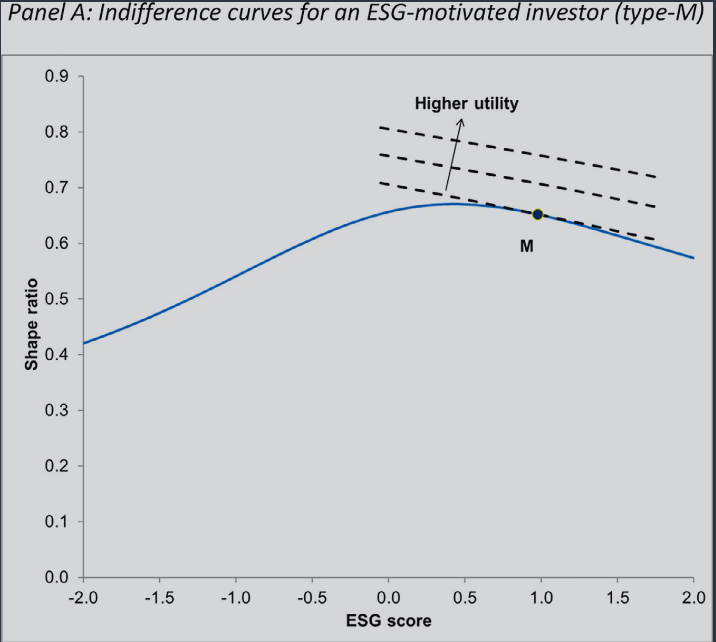
\includegraphics[width=0.45\textwidth]{./img/flammer_1.png}\hfill
    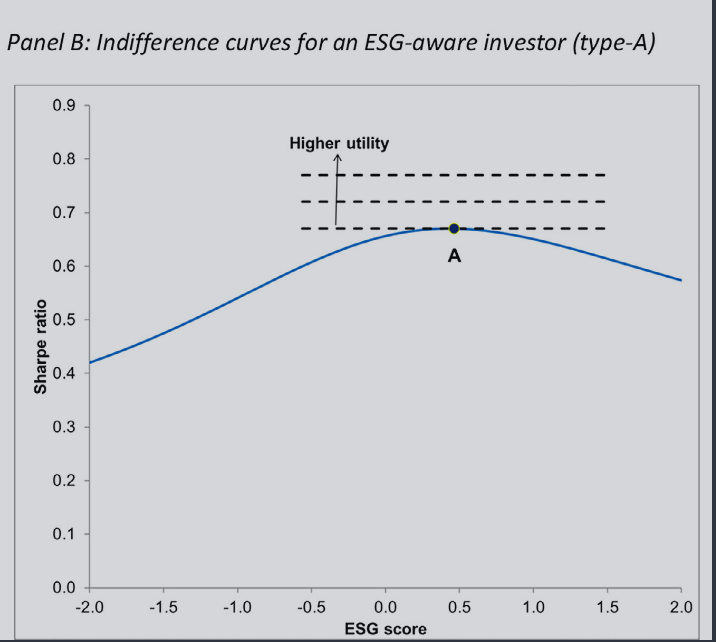
\includegraphics[width=0.45\textwidth]{./img/flammer_2.png}
\end{frame}

\begin{frame}
  \frametitle{Módszertan III.}
  A biodiverzitási prémiumot \textcite{naffa_biodiversity_2024} után határozzuk meg:
  \metroset{block=fill}
  \begin{block}{Biodiverzitási prémium (adott $\alpha$ mellett)}
  \begin{equation}
    \text{BRP}^\alpha=\text{SR}^{\alpha}_{\text{bio}} - \overline{\text{SR}^{\alpha, k}_{\text{rnd}}}
  \end{equation}
  Itt $\text{SR}^{\alpha}_{\text{bio}}$ a BIODIV-SR adott $\alpha$ biodiversity score melletti maximum elérhető Sharpe-ráta,
  $\overline{\text{SR}^{\alpha, k}_{\text{rnd}}}$ pedig $k$-szor elvégzett visszatevés nélküli mintavéttellel készített portfóliók maximum Sharpe-rátáinak átlaga.
  \end{block}
  A random generált portfólió \alert{eszközeinek számosságának mindig meg kell egyeznie} a BIODIV-SR adott pontjaihoz tartozó portfólió számosságával.
\end{frame}

\begin{frame}
  \frametitle{Kutatási kérdések}
  \begin{enumerate}
    \item A biodiverzitási preferenciával rendelkező befektetők is az egész univerzumból választanak(long vagy short), nem pedig egyszerű kizárási stratégiát alkalmaznak.\footcite{pedersen_responsible_2021} 
    \item A piaci hozamokban megjelenik-e a biodiverzitási prémium (ami elkülönül a carbon prémiumtól)\footcite{coqueret_biodiversity_2024}, és ha igen, akkor mekkora ennek a mértéke az európai piacon?\footcite{naffa_biodiversity_2024}
  \end{enumerate}
\end{frame}

\begin{frame}
  \frametitle{Adatbázisok, univerzum}
  Célunk az európai piac bemutatása, ehhez az \alert{EURO STOXX 600} indexet használjuk.\\
  \bigskip
  \metroset{block=fill}
  \begin{block}{Adatázisok}
    \begin{itemize}
    \item \alert{LSEG Refinitiv platform, új Sustainability Dashboard}: részvényárfolyamok, biodiverzitási mutatók, sustainability dashboard
    \item \alert{Bloomberg}: biodiverzitási és nature mutatók
      \item \alert{ENCORE adatbázis}: EU-ra iparágankénti nature dependency és impact mutatók
    \end{itemize}
  \end{block}
\end{frame}

\begin{frame}
    \frametitle{Adatok feldolgozása}
    Az eredeti 600 részvényhez képest \imp{555 részvény marad a kutatásunkban}. Az alábbi szűrőket alkalmaza:
    \begin{itemize}
        \item Legyen értelmezhető LSEG ESG Score Plus adat 2026-ra
        \item Legyen a részvénynek elérhető múltbéli árfolyama 2020.09.01-től 2026.09.01-ig
        \item A részvénytársaság ne USD-ben jegyezze az árfolyamát
    \end{itemize}
    \imp{Biodiverzitási mutatóink}: Biodiversity Theme Score, Biodiversity Theme Materiality Level, Biodiversity Targets, Biodiversity Impact Reduction, Biodiversity Impact Reduction Score, Biodiversity Risk Assessment, Biodiversity Risk Management Integration, Biodiversity Due Diligence
\end{frame}

\begin{frame}
    \frametitle{Egy kis ízelítő}
    Biodiversity Theme Score (elsődleges biodiverzitási mutatónk)
    \center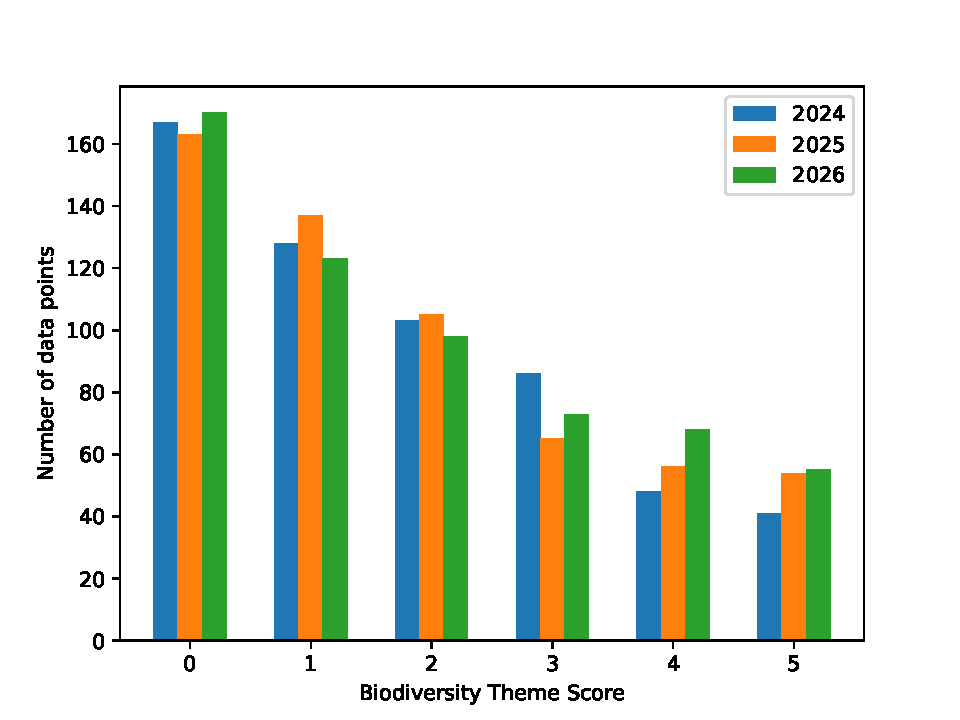
\includegraphics[width=0.6\textwidth]{../../src/plots/biodiv_theme.pdf}
\end{frame}

\begin{frame}
    \frametitle{Kockázatmentes hozam}
    \textit{Egy még nem megválaszolt kérdés, hogy mi legyen a kockázatmentes hozam?}

    -a részvények majdnem fele EUR-ben kereskedett (287), viszont ezenkívül van még 129 GBP, 62 CHF, 49 SEK, 23 DKK, 20 NOK, 17 PNL.
\end{frame}

\bibframes{Hivatkozások}
\end{document}
